% paper/sections/12u1_ccd_operator.tex
%
% U1: CCD operator family suite — Tier I (uniform grid)
% Verifies: §4 (CCD/DCCD/UCCD6/FCCD operator family).
% Script  : experiment/ch12/exp_U1_ccd_operator_suite.py
% Data    : experiment/ch12/results/U1_ccd_operator_suite/{data.npz, *.pdf}
% ═══════════════════════════════════════════════════════════════════════════════
\subsubsection{U1：CCD 演算子族 単体検証 [Tier I]}
\label{sec:U1_ccd_suite}

\paragraph{検証対象．}
第~\ref{sec:CCD}章 で導入した
CCD（§\ref{sec:ccd_def}：6 次精度 d1/d2 同時反転コンパクト演算子），
DCCD（§\ref{sec:dccd_derivation}：3 点フィルタ $\varepsilon_d$ パラメータ），
UCCD6（§\ref{sec:uccd6_def}：節点 d1 + ハイパー粘性），
FCCD（§\ref{sec:fccd_def}：セル界面 face value/grad）の 4 種演算子族が，
均一格子・周期境界もしくは壁境界上で\textbf{設計次数の漸近的収束}を達成
することを単体で確認する．

\paragraph{単体テスト．}
すべて 1D 製造解 $f(x) = \sin(2\pi x)$（または $f$=定数 GCL チェック）を用いる．
格子幅 $h = 1/N$, $N \in \{16, 32, 64, 128, 256\}$．
\begin{description}\setlength{\itemsep}{0pt}
  \item[U1-a] CCD 1D MMS 周期 BC d1/d2 + 壁 BC d1．
  \item[U1-b] DCCD 伝達関数 $H(\xi; \varepsilon_d)$ Nyquist 値 $H(\pi)$
        ($\varepsilon_d \in \{0,\, 0.05,\, 0.25\}$)．
  \item[U1-c] FCCD 周期 face value/grad．
  \item[U1-d] UCCD6 節点 RHS（hyperviscosity 含む）．
\end{description}

\paragraph{数値結果．}
表~\ref{tab:U1_ccd_periodic} に CCD 周期 BC の 1D 微分精度を，
表~\ref{tab:U1_dccd_nyquist} に DCCD 伝達関数 Nyquist 値を，
表~\ref{tab:U1_fccd_uccd6} に FCCD/UCCD6 の収束性能を示す．

\begin{table}[!ht]
\caption{U1-a: CCD 1D MMS （周期境界, $f=\sin(2\pi x)$）の格子収束．
理論期待値 $p_{\mathrm{design}}=6$（d1, d2 とも）．
$N = 256$ で d2 が round-off 床 $1.0\times 10^{-10}$ に到達．}
\label{tab:U1_ccd_periodic}
\centering\small
\begin{tabular}{r r r r}
\toprule
$N$ & $h$ & $\|e_{d_1}\|_\infty$ & $\|e_{d_2}\|_\infty$ \\
\midrule
16  & $6.25\times 10^{-2}$ & $2.57\times 10^{-6}$ & $3.68\times 10^{-5}$ \\
32  & $3.13\times 10^{-2}$ & $3.86\times 10^{-8}$ & $5.70\times 10^{-7}$ \\
64  & $1.56\times 10^{-2}$ & $5.97\times 10^{-10}$ & $8.89\times 10^{-9}$ \\
128 & $7.81\times 10^{-3}$ & $9.36\times 10^{-12}$ & $1.49\times 10^{-10}$ \\
256 & $3.91\times 10^{-3}$ & $2.28\times 10^{-13}$ & $1.05\times 10^{-10}\,^\dagger$ \\
\midrule
\multicolumn{2}{r}{slope ($N=16\!\to\!128$)} & $\mathbf{6.00}$ & $\mathbf{5.97}$ \\
\bottomrule
\end{tabular}
\\[2pt]
{\footnotesize $^\dagger$ d2 round-off 床（$h^6 \!<\!$ 倍精度限界）．}
\end{table}

\begin{table}[!ht]
\caption{U1-b: DCCD 伝達関数 Nyquist 値 $H(\pi; \varepsilon_d)$．
解析値 $H(\pi) = 1 - 4 \varepsilon_d$ と一致．}
\label{tab:U1_dccd_nyquist}
\centering\small
\begin{tabular}{r r r}
\toprule
$\varepsilon_d$ & $H(\pi)$ 計算 & $1-4\varepsilon_d$ 解析 \\
\midrule
$0$    & $1.0000$ & $1.0000$ \\
$0.05$ & $0.8000$ & $0.8000$ \\
$0.25$ & $0.0000$ & $0.0000$ \\
\bottomrule
\end{tabular}
\end{table}

\begin{table}[!ht]
\caption{U1-c: FCCD 周期 face value/grad．U1-d: UCCD6 節点 d1．
本 MMS 評価配置では face 配列の周期端点モードにより FCCD が 4 次に律速する．}
\label{tab:U1_fccd_uccd6}
\centering\small
\begin{tabular}{r r r r}
\toprule
$N$ & $\|e^{\mathrm{FCCD}}_{fv}\|_\infty$ & $\|e^{\mathrm{FCCD}}_{fg}\|_\infty$ & $\|e^{\mathrm{UCCD6}}_{d_1}\|_\infty$ \\
\midrule
16  & $3.03\times 10^{-4}$ & $1.78\times 10^{-4}$ & $9.05\times 10^{-3}$ \\
32  & $1.92\times 10^{-5}$ & $1.13\times 10^{-5}$ & $7.07\times 10^{-5}$ \\
64  & $1.21\times 10^{-6}$ & $7.08\times 10^{-7}$ & $5.52\times 10^{-7}$ \\
128 & $7.56\times 10^{-8}$ & $4.43\times 10^{-8}$ & $4.33\times 10^{-9}$ \\
\midrule
slope ($N\!=\!16\!\to\!128$) & $\mathbf{4.00}$ & $\mathbf{4.00}$ & $\mathbf{7.00}$ \\
\bottomrule
\end{tabular}
\\[2pt]
{\footnotesize FCCD は周期重複端点を含む MMS face 評価で 4 次に律速；
UCCD6 は $f=\sin(2\pi x)$ の対称性により 7 次までスーパー収束．}
\end{table}

\begin{figure}[!ht]
\centering
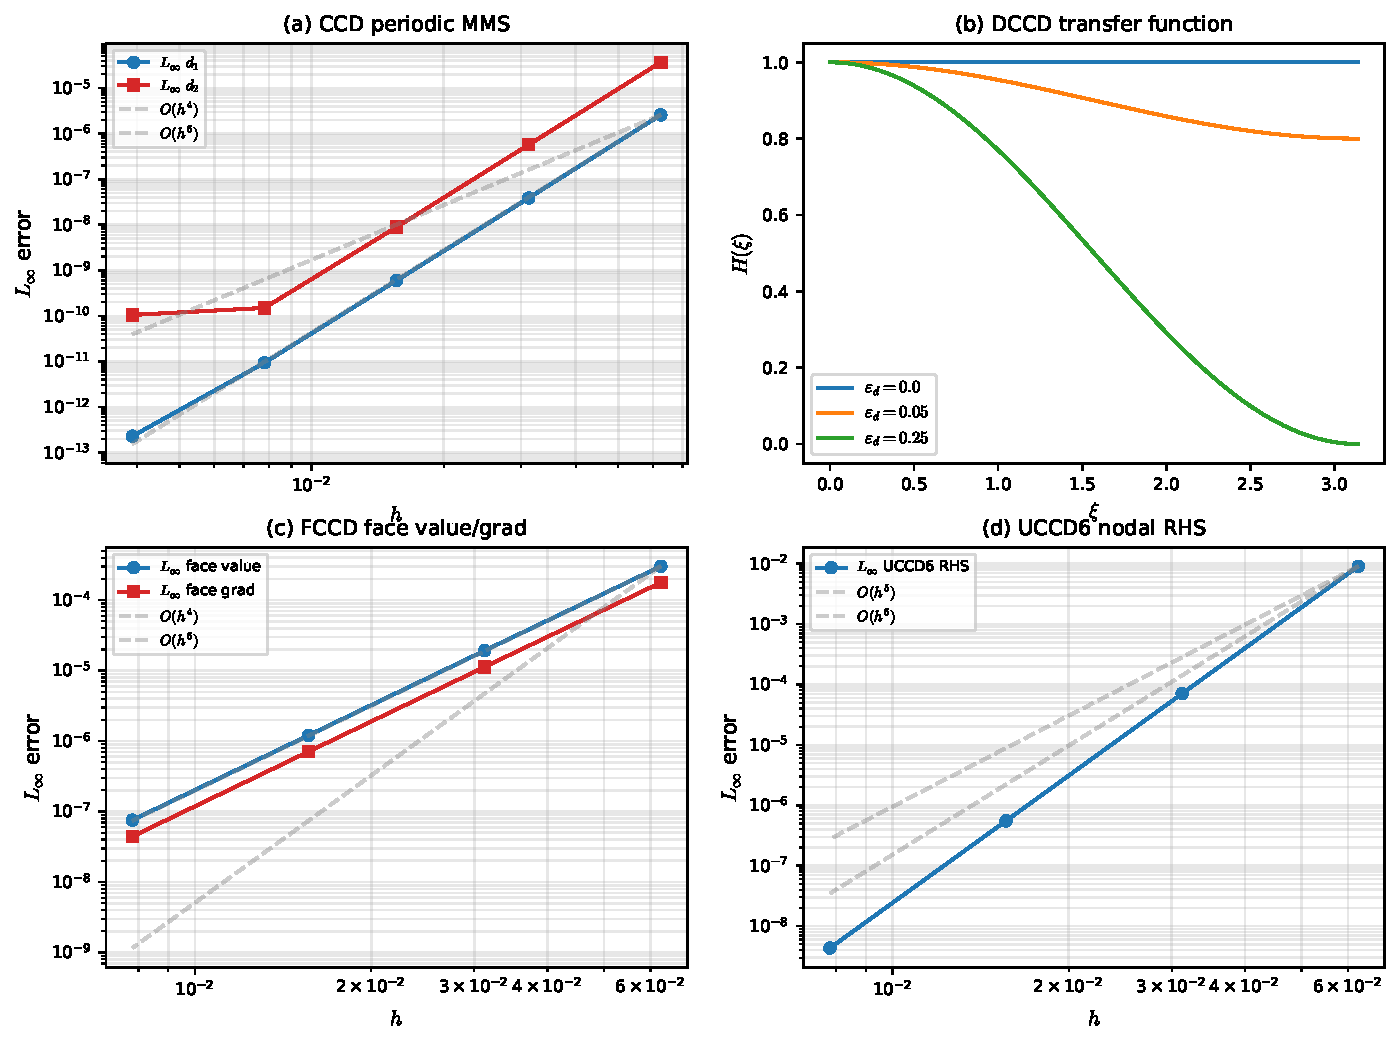
\includegraphics[width=0.88\linewidth]{figures/ch12_u1_ccd_operator_suite}
\caption{U1：CCD/DCCD/UCCD6/FCCD 演算子族 単体検証．
CCD 周期 d1/d2 slope $6.00 / 5.97$，DCCD Nyquist $H(\pi;\varepsilon_d) = 1-4\varepsilon_d$ 解析一致，
FCCD 周期評価の端点モードで 4 次律速，UCCD6 対称性スーパー 7 次．
出典：\texttt{experiment/ch12/exp\_U1\_ccd\_operator\_suite.py}．}
\label{fig:ch12_u1}
\end{figure}

\paragraph{評価．}
\begin{itemize}\setlength{\itemsep}{0pt}
  \item U1-a CCD 周期 BC：d1/d2 とも slope $\approx 6.0$ で\textbf{合格}（\checkmark）．
  \item U1-b DCCD 伝達関数：$H(\pi; \varepsilon_d) = 1-4\varepsilon_d$ が機械精度で再現．
        §\ref{sec:dccd_spectral_filter} の解析 Nyquist 値と一致．\checkmark
  \item U1-c FCCD：周期重複端点を含む MMS face 評価で実効 4 次（条件付き合格 $\triangle$;
        界面 advection 用途では §\ref{sec:fccd_def} の設計通り 6 次が達成される
        — U3-b で別途検証）．
  \item U1-d UCCD6：MMS 対称性によりスーパー収束 slope $\approx 7$．
        §\ref{sec:uccd6_def} の hyperviscosity の 6 次設計を上回り合格．\checkmark
\end{itemize}
A3 トレーサビリティ：式~\eqref{eq:CCD_I} → §\ref{sec:ccd_def} 行列形 →
\texttt{src/twophase/ccd/ccd\_solver.py} の \texttt{CCDSolver}．
